\setauthor{Raffeiner Christine}
\section{Zusammenfassung}
Ergebnis der Arbeit ist eine lauffähige Applikation bestehend aus Frontend, Backend, Keycloak und Datenbank.
Alle Komponenten wurden gelockert und auf eine VM deployed. Für die Sicherheit sorgt eine Sperre der Ports für die VM und der 
Reverse-Proxy Traefik.

\section{Frontend}
Es folgen Abbildung der wichtigsten Unterseiten und Funktionalitäten der Arbeit. \cite{noauthor_felx-box_nodate}, \cite{noauthor_w3schools_nodate}, \cite{noauthor_wait_nodate}
\begin{figure}[H]
    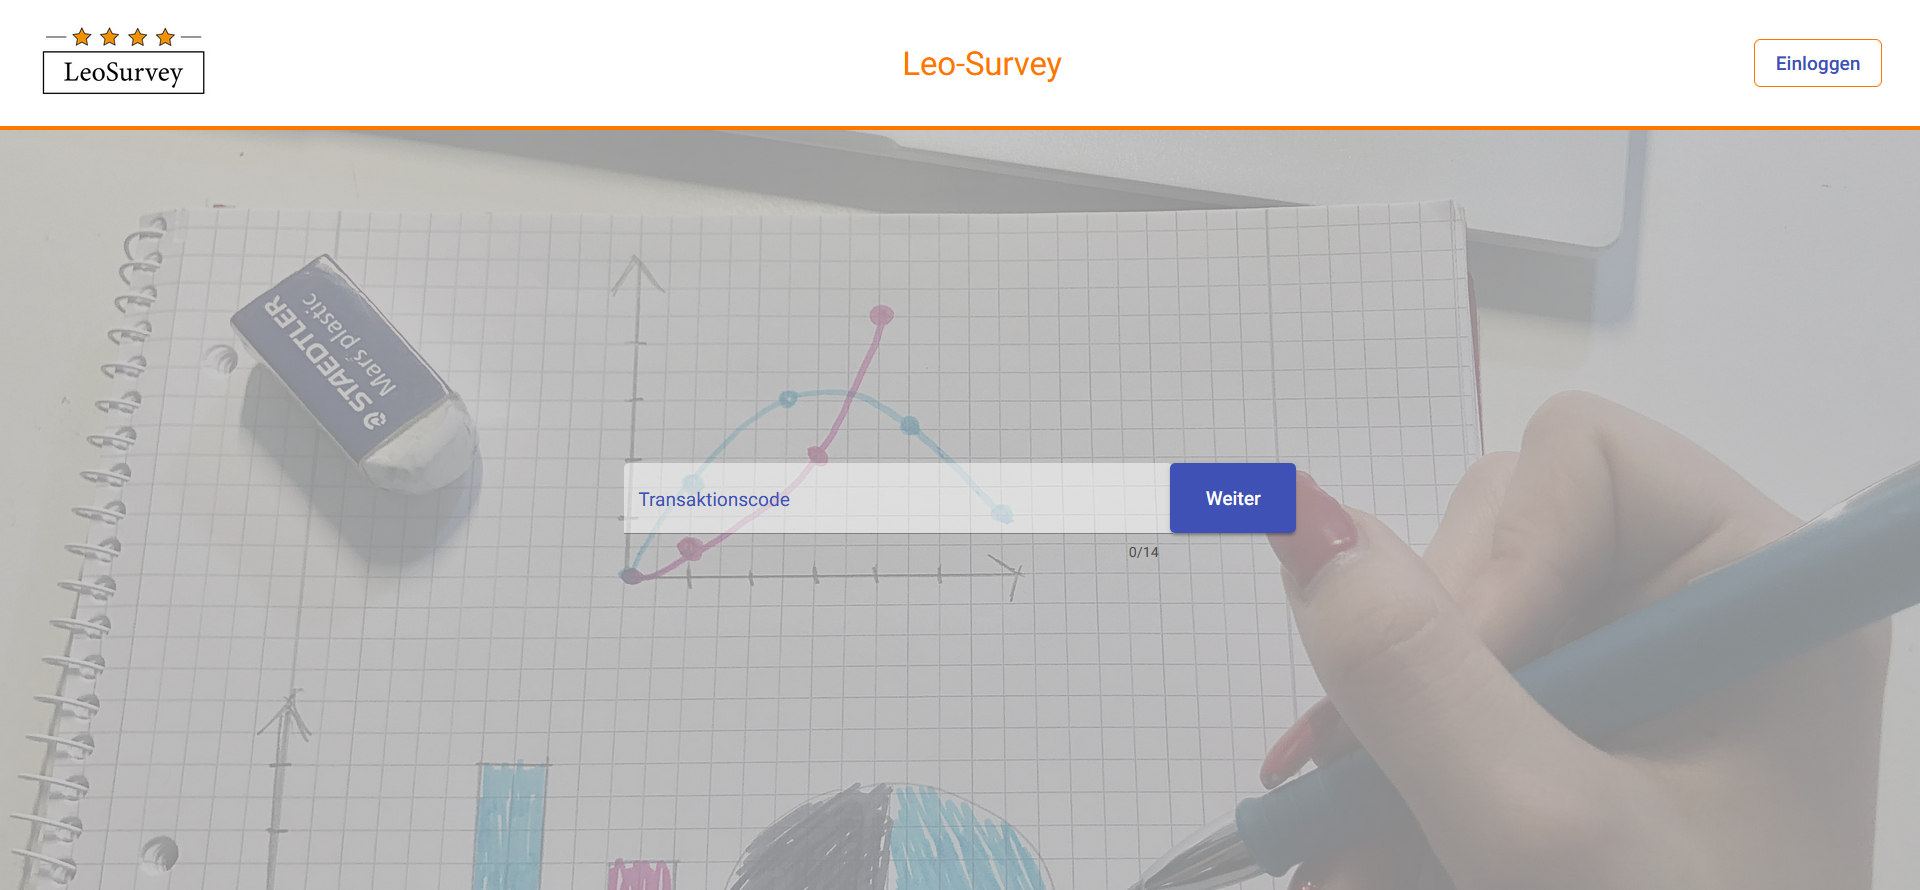
\includegraphics[width=0.9\textwidth]{pics/Ergebnis_Startseite.PNG}
    \centering
    \caption{Startseite}
\end{figure}

\begin{figure}[H]
    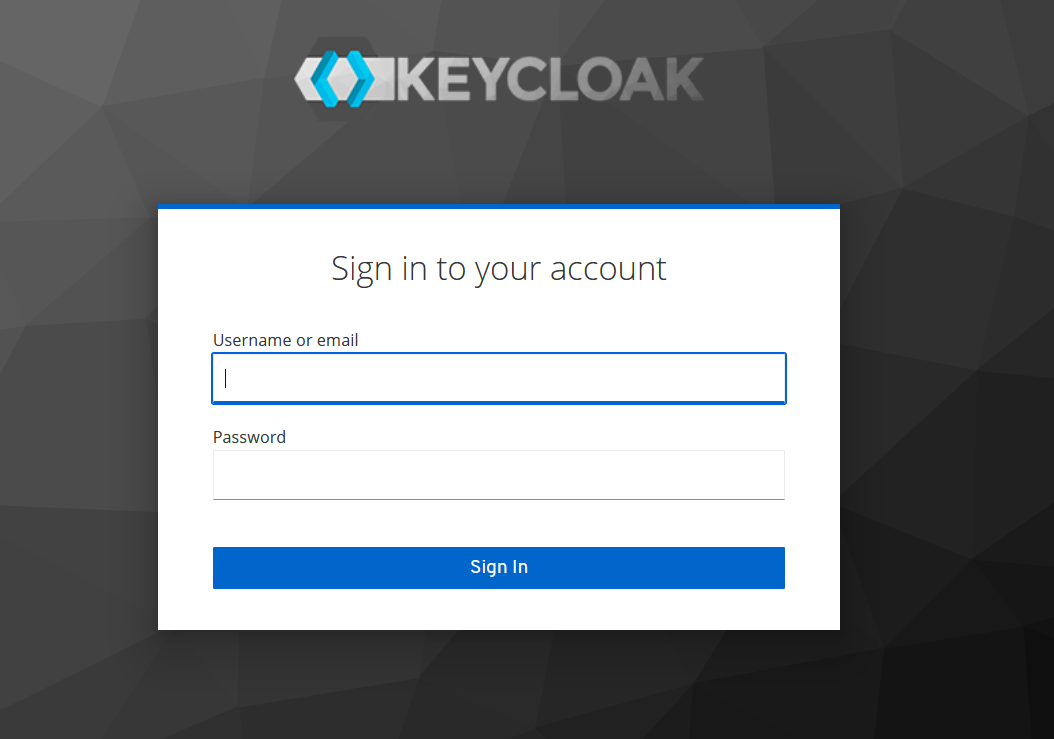
\includegraphics[width=0.9\textwidth]{pics/Ergebniss_KC.PNG}
    \centering
    \caption{Login mittels Keycloak}
\end{figure}
Mithilfe des Keycloak können sich die Schüler/innen und Lehrer/innen mit dem gewohnten Anmeldedaten anmelden.   

\begin{figure}[H]
    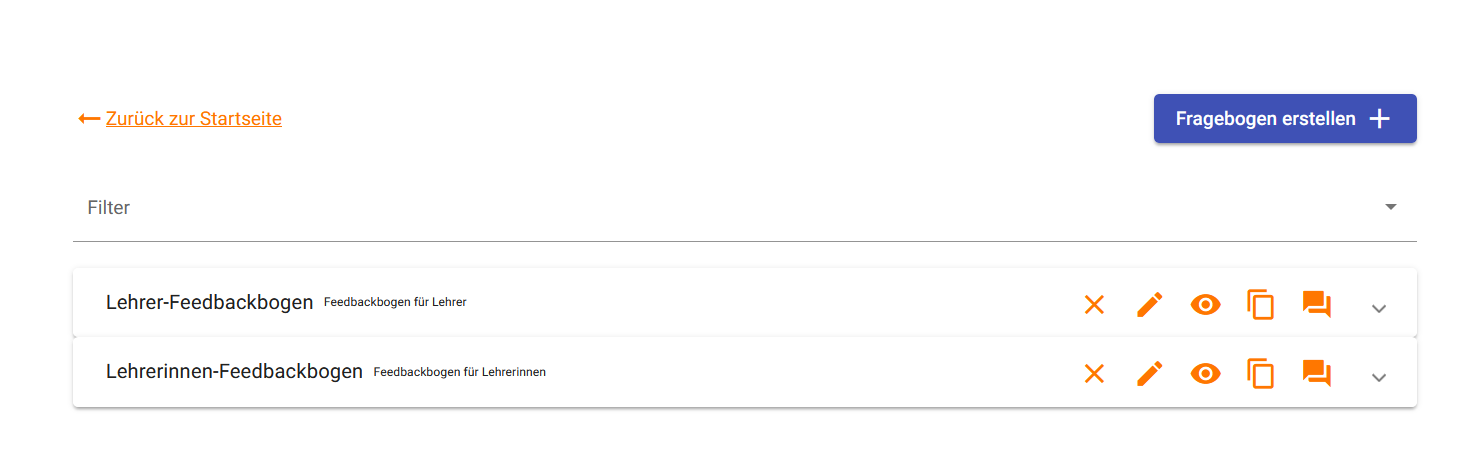
\includegraphics[width=0.9\textwidth]{pics/Ergebnis_Dashboard.PNG}
    \centering
    \caption{Dashboard}
\end{figure}

Auf dem Dashboard werden alle für den / die Benutzer/in verfügbaren Fragebögen und Umfragen angezeigt.
Alle Fragebögen und Umfragen, die im Besitz einer Person sind, können geändert und gelöscht werden. Von anderen Fragebögen können 
Kopien erstellt werden. Fragebögen können gefiltert werden. Umfragen können erstellt und ausgewertet werden.

\begin{figure}[H]
    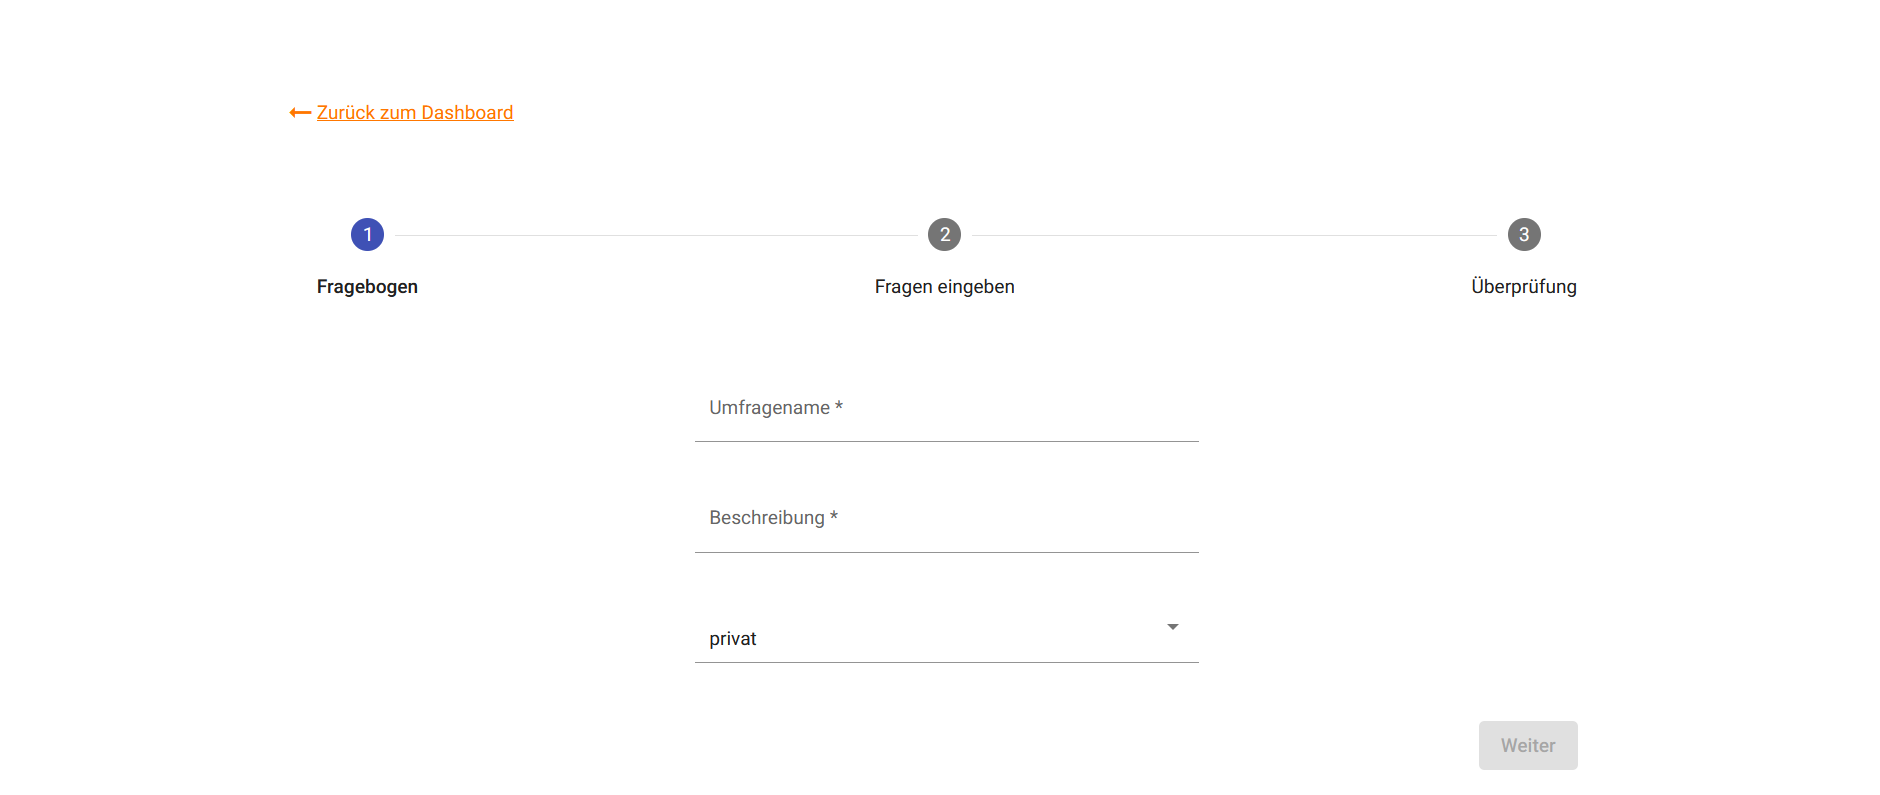
\includegraphics[width=0.9\textwidth]{pics/Ergebnis_Erstellen.PNG}
    \centering
    \caption{Fragebogen erstellen}
\end{figure}

\begin{figure}[H]
    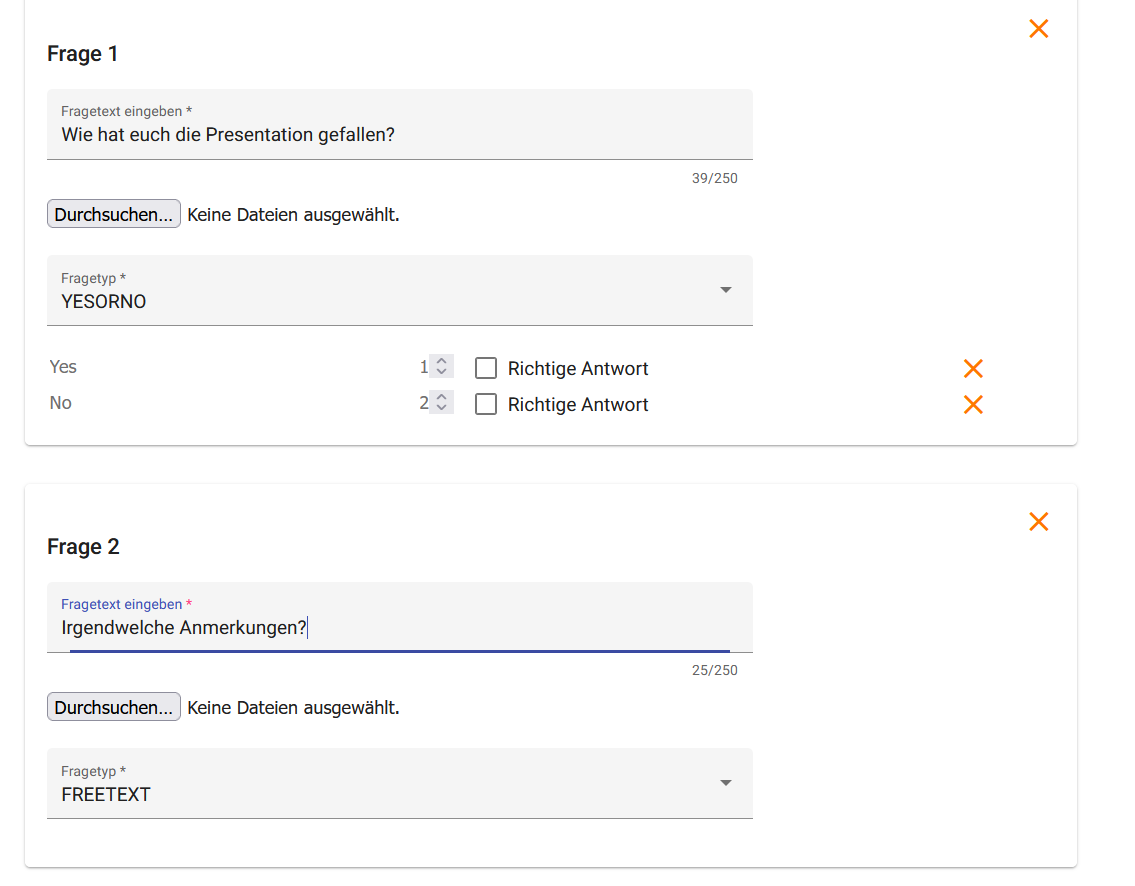
\includegraphics[width=0.9\textwidth]{pics/Ergebnis_Erstellen2.PNG}
    \centering
    \caption{Startseite}
\end{figure}

Fragebögen können stufenweise erstellt werden. Es kann zwischen vier verschieden Fragetypen gewählt werden.

\begin{figure}[H]
    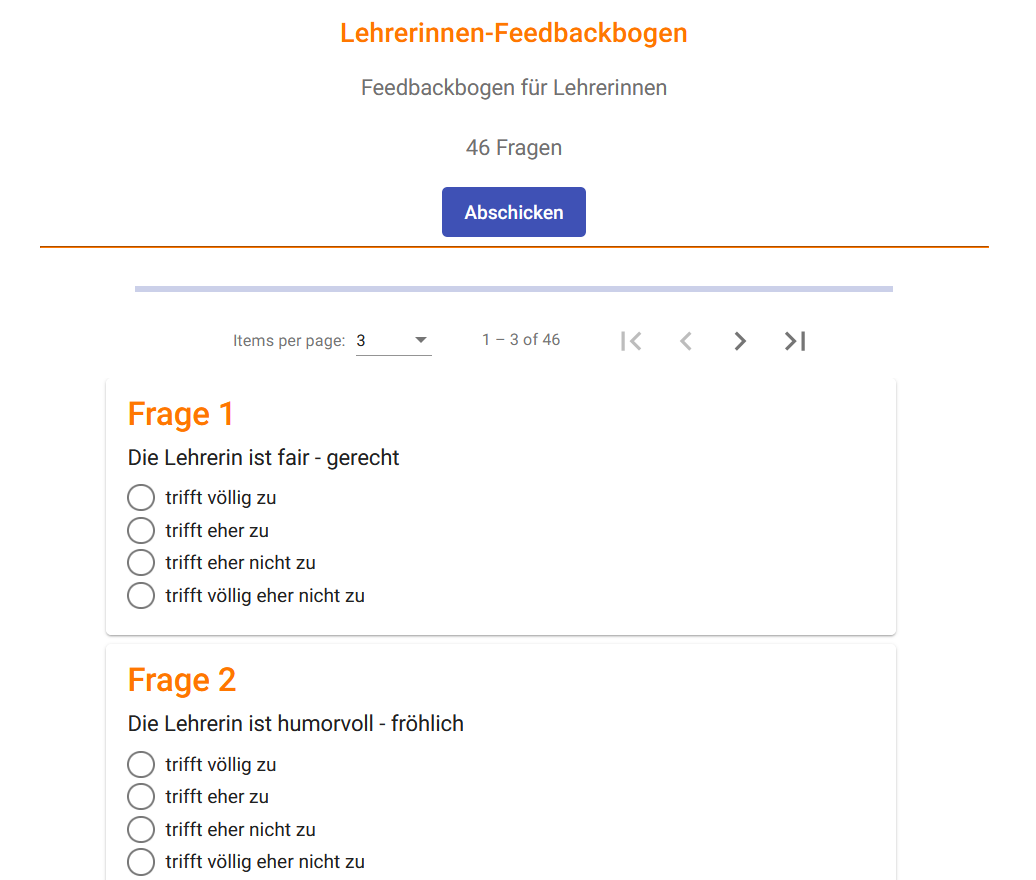
\includegraphics[width=0.9\textwidth]{pics/Ergebnis_Antworten.PNG}
    \centering
    \caption{Startseite}
\end{figure}

Das Beantworten der Umfrage erfordert keinen Login und wird mithilfe von Transaktionscodes durchgeführt. 
Fragen werden in kleinen Gruppen zusammengefasst, angezeigt und können optional beantwortet werden. 
Vor dem Abschicken wird dem/er Benutzer/in angezeigt, wie viele Fragen er / sie nicht beantwortet hat.